\chapter{Background Theory}

  \section{Authentication}

  Authentication is the process of verifying whether a particular individual or a device should be granted access to a system or application running on a device \cite{IPAS}, e.g. verifying that you are the person that you claim to be.

  There are various authentication schemes described in the literature, but they can all be grouped by the following characteristics \cite{IPAS}:

    \begin{itemize}
      \item Who you are
      \item Something you have, and
      \item Something you know
    \end{itemize}

    \subsection{Biometric Authentication}
    Biometric authentication have the characteristics of ``who you are''. Biometric authentication refers to verify a persons identity based on physical or behavioral characteristics of an individual \cite{biometrics, biometrics2}. Biometric authentication are different than other authentications schemes because:

      \begin{itemize}
        \item the biometric password cannot be lost nor forgotten
        \item biometric passwords tends to be difficult to copy, share and distribute, and 
        \item the person being authenticated needs to be present in the authentication process
      \end{itemize} 

     Physiological biometrics uses the physiological characteristics of an individual in the authentication process. The verification uses unique characteristics of a human, e.g. physical parts of the body that are unique like fingerprints, face, iris, hand and finger geometry, and DNA. Behavioral biometrics analyze how a person performs different activities, e.g. applies pattern recognition techniques for activities like keyboard writing, talking and handwriting.

    \subsection{Token-based Authentication}
    In a token-based authentication process the user uses ``something you have'' that is often stored on a physical device. Token-based authentication is often combined with a ``something you know'', making a strong authentication by combining two or more authentication characteristics. In many banking systems you have to use more than just something you know, but also ``something you have'', like a one-time password to pass the authentication process. The one time password is a password that is randomly generated and sent to a physical device, or over an SMS to your mobile phone. This is an extra layer of security, because even if someone steals or know your password, they still cant get access to your banking account because they also would need your security token.

    \subsection{Knowledge-based Authentication}
    ``Something you know'' is often used in the classical login situation where the user have to remember a username/password to get access to a system or device. Some of the commonly used passwords schemes are PIN's, alphanumeric passwords and graphical passwords that all are passwords with the characteristic of ``something you know''.

      {\bf PIN's} Personal identification number is a numeric passwords. The PIN was first introduced in the first ATM in London in 1967 as a efficient way for the banks to authenticate their customers \cite{Bonneau1}.      

      {\bf Alphanumeric passwords}
      The word ``Alphanumeric'' is a composition of the words ``alpha'' (as in alphabet), and ``numeric''(as in numbers). The alphanumeric password may also contain special characters, so in short a alphanumeric password is a mix of all writable characters.

      {\bf Graphical passwords}
      A graphical password have the characteristics of ``something you know'', but instead of using letters and numbers it uses graphical elements as a secret. Graphical passwords was proposed as a alternative to PINs and alphanumeric values because humans tends to remember graphical elements better than letters and numbers. A variety of graphical passwords schemes have been created over the past years. Biddle et al. have collected research of the past decade on graphical password schemes \cite{Biddle}, dividing the schemes into three categories: 

      \begin{itemize}
        \item Recall-based authentication
        \item Recognition-based authentication, and 
        \item Cued-recall authentication.
      \end{itemize}

      Recall-based graphical passwords are often referred to as drawmetric systems \cite{DeAngeli} because the user are are reproducing a secret drawing. The password is normally drawn in a grid or a blank canvas, requiring the user to reproduce the secret password from its memory.

      Recognition-based passwords are often referred to as cognometric systems \cite{DeAngeli} because the user recall a secret drawing, or sequence of drawings, and the reproduces it as the secret password.

      Cued-recall are often referred to locimetric systems \cite{DeAngeli}. With cued-recall authentication typically require the users to remember and target a specific location within and image. This is a version of a recall-based authentication, but helps the user with the recall by showing an image and not just an grid or canvas. It is also different from the recognition-based approach because the user need to identify specific locations in an image as a whole. 

  \section{Key Security Aspects in Authentication}

  In order to be able to evaluate the security of different password schemes, this section will give a brief introduction to key security aspects with knowledge-based authentication, hereafter called passwords.In terms of security, the primary goal of authentication is to provide security for its intended environment in order to avoid security attacks. A password, regardless of format, is a secret a user needs to use in order to to grant access to a system or device. A password should have certain features in order to be secure:

    \begin{itemize}
      \item The password should be hard to guess, meaning that the password should have a high entropy,
      \item The password should be easy to remember for users, and 
      \item The password should remain a secret for the intended user.
    \end{itemize}

  When we talk about security, we often talk about if a password scheme is ``crackable'', meaning that the a password are guessable. When a password scheme is measured to be ``hard to guess'', it is normal to measure the strength of the password scheme in terms of its entropy. The password strength is measured in terms of information entropy, measured in bits. Instead of measuring the security of a password in number of guesses needed to guess the password, we use the base-2 logarithm of the number of guesses, which is the number of ``entropy bits'' in a password. We use the notation L for the length of the symbols in the password, and they are chosen from a set of N possible symbols. The formula for password entropy are:

    \begin{equation}
      Password Entropy = log_{2}(N^{L})
    \end{equation}

  When we say that a password scheme is easy to use it is normal to measure the success rate when writing and remembering a password, e.g. how long it takes for users to write and remember their passwords. When a password is easy to remember, it often refers to a password schemes ability to maintain its usability. As stated, a password that have a higher entropy are harder to guess, but are often obtained by making long passwords. It is well known that humans have a hard time remembering long and complex passwords. Therefore it is important that a password scheme are supporting the users to make passwords that they can remember, and also are secure. 

  When users make their password it should only remain a secret that the intended user know about. A password scheme that lack support of usability often make people do actions like make simple passwords that are easy to remember, but also easy to guess, or even write down and use the same passwords across multiple systems. 

  All of the key security aspects are important to understand when you are studying password mechanisms. The key aspects will be used throughout this thesis in order to be able to evaluate and read research focusing passwords. 

  \section{Shortcomings With Text-Based Authentication} 

%\cite{DejaVu}
  User authentication is a central component of security systems. In order to get access to systems you need to pass a authentication process. Despite the large number of options for authentication, text-based passwords remain the most common authentication scheme. The reason why they are widely adopted is because they are easy and inexpensive to implement, and users are familiar with the scheme. It is also avoiding the privacy issues raised by biometric authentication and avoid the need for bringing a physical security device that are used in token-based authentication schemes. However, text-based authentication suffer from both security and usability disadvantages. Today, users needs to remember an increasingly number of password, making users to adopt bad password habits. 

  The term ``habit'' is often a bad thing when talking about security. A habit is often hard to change and are often a predictable pattern. Password reuse is one of the known password habits among users because the human limitation to remembering text-based password. Some users also make simple or meaningful password that are easier to remember, making their passwords vulnerable to attacks. It is a well known problem that users tends to have an increasingly number of accounts that requires the users to remember yet another number of password across multiple systems and devices. The problem is not just to remember all the password needed, but also remembering which passwords that belongs to which account or device. Because of the human capacity of remembering password are causing users to choose weak passwords, as well as reuse the passwords across multiple web pages. In order to understand the shortcomings with text-based passwords, this section will include relevant research on users choices on text-based passwords.  

  \begin{wrapfigure}{l}{0.4\textwidth}
    \vspace{-20pt}
    \begin{center}
      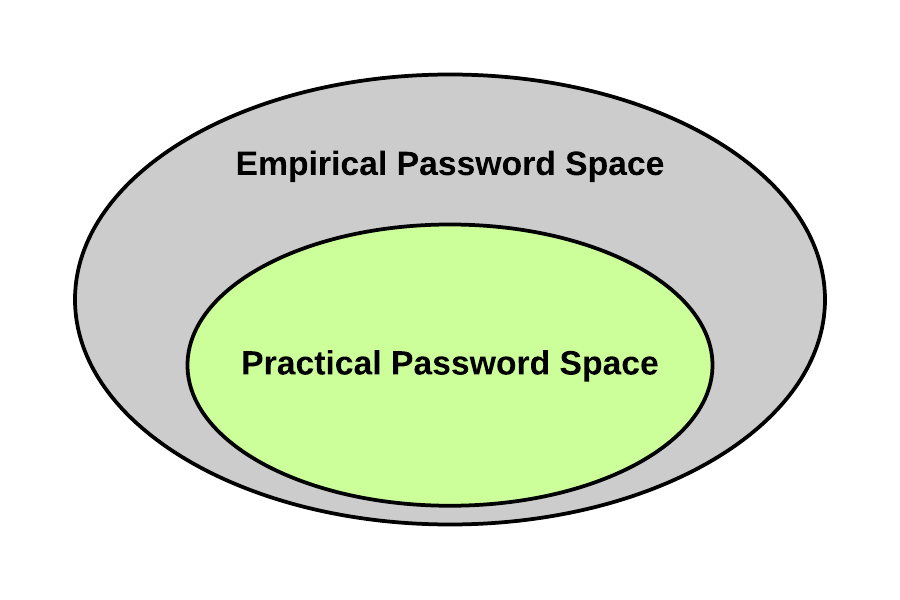
\includegraphics[scale=0.16]{pics/EmpiricalVsPractical.png}
    \end{center}
    \vspace{-20pt}
    \caption{Empirical vs. Memorable Password Space}
    \vspace{0pt}
  \end{wrapfigure}

  Password schemes have what is called an empirical password space, that is the number of possible passwords that a user can make. The problem with many password schemes is that it seems that users don't tend to use the full password space, but only a subset of the possible passwords, e.g. the memorable password space, making the memorable password space less than the empirical password space. This shows that the security of a password scheme is linked closely to is memorable password space rather than its full password space.

  In a case study of 14.000 Unix passwords, a research group found a 25\% of the passwords were in a group of words forming a dictionary of $3\times10^{6}$ words \cite{UnixPasswords}. This dictionary shows that an attacker can have a relatively high success rate with an attack, despite the fact that there a roughly $2\times10^{14}$ 8-character passwords consisting of digits, and upper case and lower case letters. Due to the limitations of human memory, users often choose passwords which are easier to remember, causing a significant number of user-chosen password to fall into a small dictionary, e.g. practical password space \cite{Tao}. A well-designed dictionary is a tiny subset of the full password space, e.g. theoretical password space, which further can be prioritized  according to the likelihood for a password to be chosen. It is therefore a commonly stated that the security of a password scheme is related closely to the size of its memorable/practical password space, rather than its theoretical password space. The high success rate of dictionary attack against textual passwords is believed to be strongly related to the recall capabilities of humans and how they choose their passwords, e.g. making meaningful and thus more easily remembered words are chosen as passwords. 

  One of the first large-scale studies on web password habits was conducted in 2007 by Microsoft research \cite{habits1}. They analyzed web password habits among 544960 web users over a period of 3 months. The data was collected from a Windows Live Toolbar and they observed activities like login frequency. They also collected information about the users age, the strength of the users passwords, as well as number of unique passwords and its use across different URLs. They observed that a normal user have an average of 7 distinct password and that an average of 5 of these password was re-used on different web pages. The estimate on average number of account pr user was estimated to be 25 account pr user, but this would probably be higher since it 7 years ago. 

  {\color{red} \bf WRITE SOMWTHING MORE??}

  %REWRITE!!!
  Because of the shortcomings with text-based authentication, graphical authentication are getting getting increased attention because it are an alternative to text-based authentication trying to cope with the memorability and security issues of text-based password.
   



 %  \section{Passphrase and PIN's vs. graphical passwords}
 %  \section{A password are more then just a password}

 %    If you take a walk in the street and ask a random person ``what is a password?'', 
 %    you probably get the aswer ``its letters and digits''. Passwords are so much more than just letter and digits. 

 %    Nowadays everything we do require you to keep this secret called a password. Your work, you're social life, 
 %    even you're private life is forcing you to keep track of passwords. How do you keep track of all of them?
 %    You probably keep the same password at many places. 
 %    \subsection{Theoretical Password Space}
 %    \subsection{Practical Password Space}

 %  \section{Relevant Data Collection Methods}
 %    In this section I will explore different methods for collecting data. It will give a brief summary of the 
 %    method as well as summary and discussion of the different methods at the end. 
 %    \subsection{Android Unlock Patterns Games}
 %    \subsection{Relevant User Studies}
 %    \subsection{Summary of Methods}
 %  \section{Information gathering}
	% \section{Psycology and passwords}
	% \section{Graphical passwords}
	% \section{Android Unlock Pattern}
